\artigofalse
\chapter{R-PACKAGE SPSANN: OPTIMIZATION OF SAMPLE CONFIGURATIONS USING SPATIAL SIMULATED ANNEALING}
\shorttitle{Package \texttt{spsann} for \texttt{R}}
\label{apen:spsann}

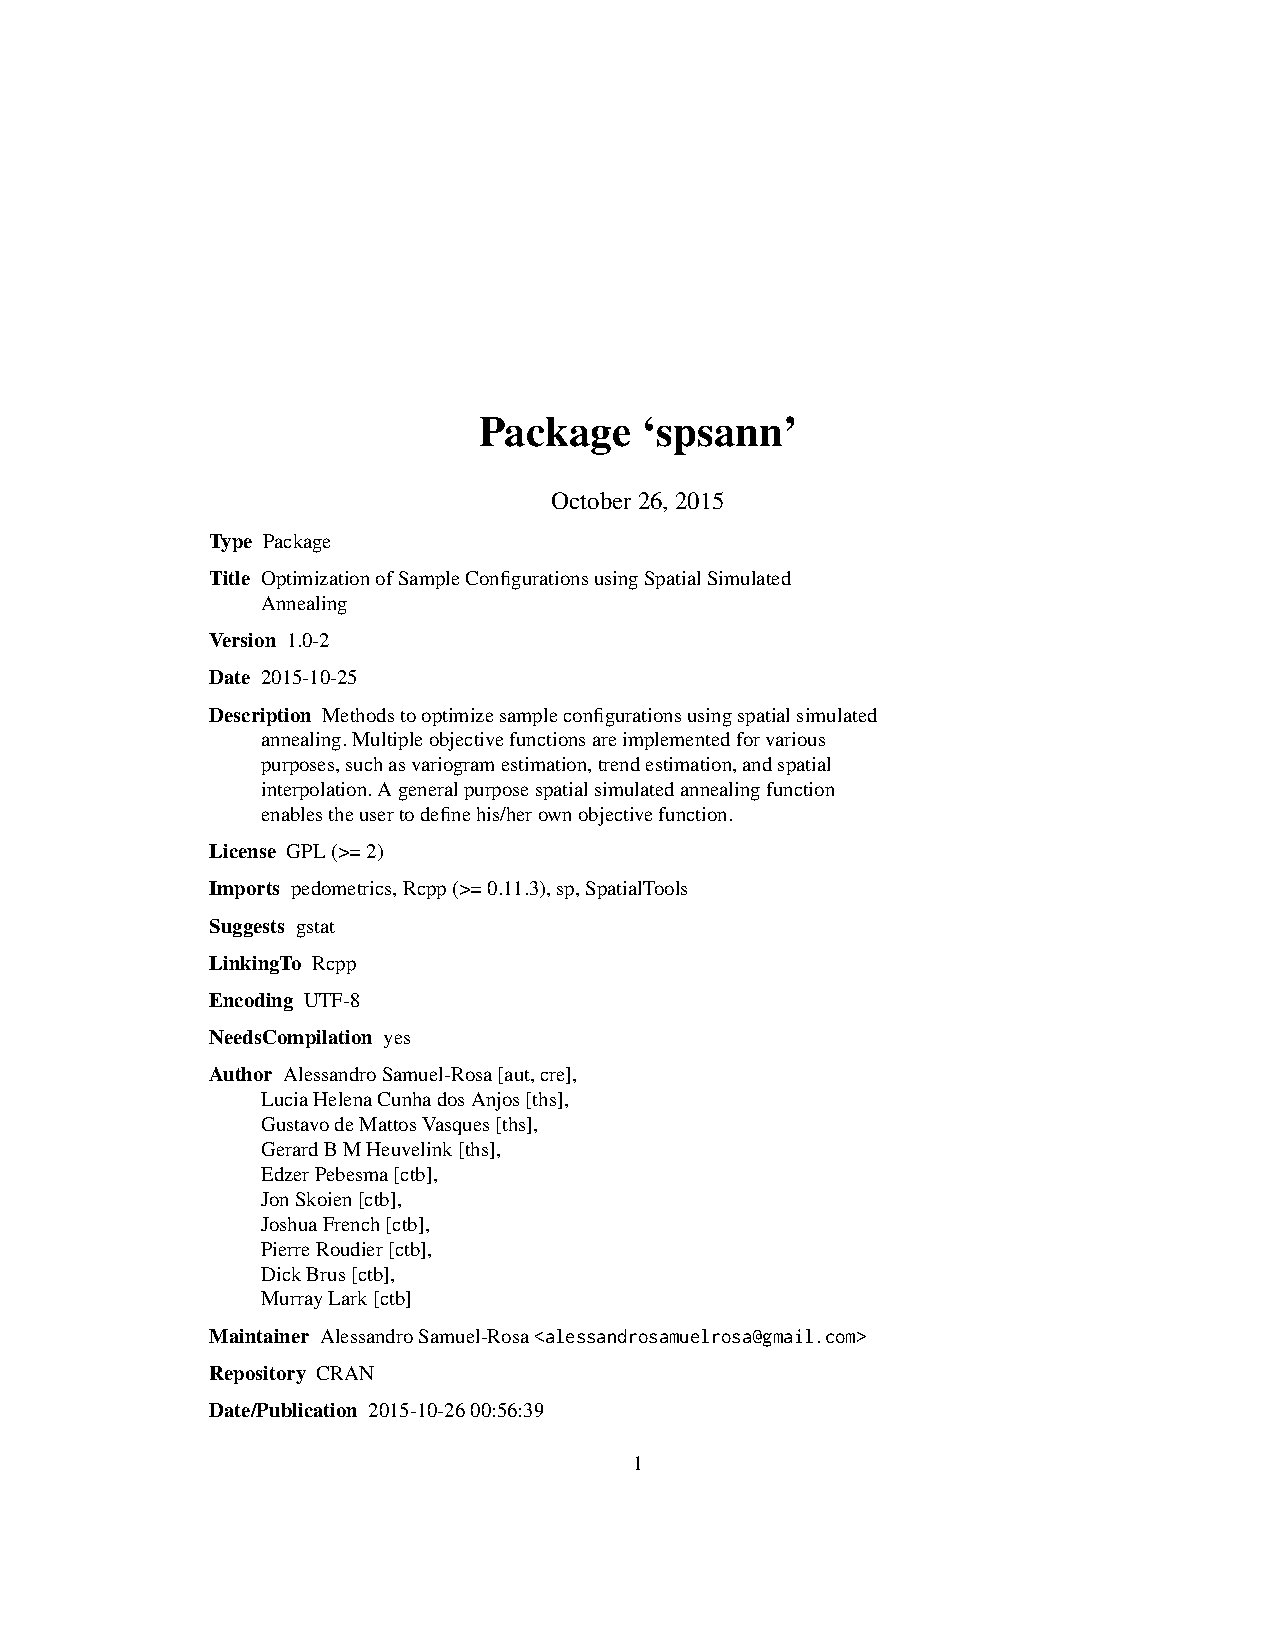
\includepdf[pages=-, width=1.2\textwidth]{chap/spsann.pdf}

% \section{Objective functions}
% 
% \subsection{Spatial trend identification and estimation}
% 
% \subsubsection{DIST}
% 
% Reproducing the marginal distribution of the numeric covariates depends upon
% the definition of marginal sampling strata. These marginal sampling strata 
% are also used to define the factor levels of all numeric covariates that  
% are passed together with factor covariates. Two types of marginal sampling 
% strata can be used: \textit{equal-area} and \textit{equal-range}.
% 
% \textit{Equal-area} marginal sampling strata are defined using the sample 
% quantiles estimated with the \texttt{quantile}-function of the 
% \textbf{stats}-package using a discontinuous function (\texttt{type = 3}). This 
% is to avoid creating breakpoints that do not occur in the population of 
% existing covariate values.
% 
% Depending on the level of discretization of the covariate values, 
% the \texttt{quantile}-function produces repeated breakpoints. A breakpoint 
% will be repeated if that value has a relatively high frequency in the 
% population of covariate values. The number of repeated breakpoints increases 
% with the number of marginal sampling strata. Repeated breakpoints result in
% empty marginal sampling strata. To avoid this, only the unique breakpoints 
% are used.
% 
% \textit{Equal-range} marginal sampling strata are defined by breaking the range
% of covariate values into pieces of equal size. Depending on the level of 
% discretization of the covariate values, this method creates breakpoints that
% do not occur in the population of existing covariate values. Such breakpoints
% are replaced by the nearest existing covariate value identified using 
% Euclidean distances.
% 
% Like the equal-area method, the equal-range method can produce empty marginal
% sampling strata. The solution used here is to merge any empty marginal 
% sampling strata with the closest non-empty marginal sampling strata. This is
% identified using Euclidean distances as well.
% 
% The approaches used to define the marginal sampling strata result in each 
% numeric covariate having a different number of marginal sampling strata, 
% some of them with different area/size. Because the goal is to have a sample 
% that reproduces the marginal distribution of the covariate, each marginal 
% sampling strata will have a different number of sample points. The wanted 
% distribution of the number of sample points per marginal strata is estimated 
% empirically as the proportion of points in the population of existing 
% covariate values that fall in each marginal sampling strata.
% 
% \subsubsection{CORR}
% 
% The \textit{correlation} between two numeric covariates is measured using the 
% Pearson's \textit{r}, a descriptive statistic that ranges from $-1$ to $+1$. 
% This statistic is also known as the linear correlation coefficient.
% 
% When the set of covariates includes factor covariates, all numeric covariates 
% are transformed into factor covariates. The factor levels are defined 
% using the marginal sampling strata created from one of the two methods 
% available (equal-area or equal-range strata).
% 
% The \textit{association} between two factor covariates is measured using the 
% Cramér's \textit{v}, a descriptive statistic that ranges from $0$ to $+1$. The 
% closer to $+1$ the Cramér's \textit{v} is, the stronger the association between 
% two factor covariates. The main weakness of using the Cramér's \textit{v} is 
% that, while the Pearson's \textit{r} shows the degree and direction of the 
% association between two covariates (negative or positive), the Cramér's 
% \textit{v} only measures the degree of association (weak or strong).
% 
% \subsection{Variogram identification and estimation}
% 
% PPL: points and pairs; minimum and distribution
% 
% \subsection{Spatial interpolation}
% 
% MKV and MSSD
% 
% \subsection{Multi-objective optimization}
% 
% ACDC: CORR and DIST;
% CLHS;
% SPAN: CORR, DIST, PPL, and MSSD;
% 
% A method of solving a multi-objective optimization problem is to aggregate 
% the objective functions into a single \textit{utility function}. In the
% \textbf{spsann}-package, the aggregation is performed using the \textit{weighted 
% sum method}, which incorporates in the weights the preferences of the user 
% regarding the relative importance of each objective function.
% 
% The weighted sum method is affected by the relative magnitude of the 
% different function values. The objective functions implemented in the
% \textbf{spsann}-package have different units and orders of magnitude. The 
% consequence is that the objective function with the largest values will have 
% a numerical dominance in the optimization. In other words, the weights will 
% not express the true preferences of the user, and the meaning of the utility 
% function becomes unclear.
% 
% A solution to avoid the numerical dominance is to transform the objective
% functions so that they are constrained to the same approximate range of 
% values. Several function-transformation methods can be used and the 
% \textbf{spsann}-package offers a few of them. The \textit{upper-lower-bound 
% approach} requires the user to inform the maximum (nadir point) and minimum 
% (utopia point) absolute function values. The resulting function values will 
% always range between 0 and 1.
% 
% Using the \textit{upper-bound approach} requires the user to inform only the
% nadir point, while the utopia point is set to zero. The upper-bound approach
% for transformation aims at equalizing only the upper bounds of the objective 
% functions. The resulting function values will always be smaller than or equal
% to 1.
% 
% Sometimes, the absolute maximum and minimum values of an objective function 
% can be calculated exactly. This seems not to be the case of the objective 
% functions implemented in the \textbf{spsann}-package. If the user is 
% uncomfortable with informing the nadir and utopia points, there is the option
% for using \textit{numerical simulations}. It consists of computing the 
% function value for many random sample configurations. The mean function 
% value is used to set the nadir point, while the the utopia point is set to
% zero. This approach is similar to the upper-bound approach, but the function
% values will have the same orders of magnitude only at the starting point of 
% the optimization. Function values larger than one are likely to occur during 
% the optimization. We recommend the user to avoid this approach whenever 
% possible because the effect of the starting point on the optimization as a 
% whole usually is insignificant or arbitrary.
% 
% The \textit{upper-lower-bound approach} with the \textit{Pareto maximum and 
% minimum values} is the most elegant solution to transform the objective 
% functions. However, it is the most time consuming. It works as follows:
% 
% \enumerate{
%   \item Optimize a sample configuration with respect to each objective
%   function that composes the MOOP;
%   \item Compute the function value of every objective function that composes 
%   the MOOP for every optimized sample configuration;
%   \item Record the maximum and minimum absolute function values computed for 
%   each objective function that composes the MOOP -- these are the Pareto
%   maximum and minimum.
% }
% 
% For example, consider that a MOOP is composed of two objective functions: A 
% and B. The minimum absolute value for function A is obtained when the sample
% configuration is optimized with respect to function A. This is the Pareto
% minimum of function A. Consequently, the maximum absolute value for function
% A is obtained when the sample configuration is optimized regarding function
% B. This is the Pareto maximum of function A. The same logic applies for 
% function B.
% 
% \section{Generation mechanism}
% 
% The \textit{generation mechanism} corresponds to the set of formal rules used 
% to randomly perturb the sample configuration to create a new solution out of the
% current one. This is done by adding random noise to the coordinates of one of 
% the sample points, a process known as \textit{jittering}.
% 
% Before we jitter a given sample point, we have to define the maximum quantity 
% of random noise that can be added to its coordinates, i.e. the area within 
% which it can be moved around. In principle, this area corresponds to a rectangle
% centred at the sample point that ignores the presence of non-sampling areas 
% (e.g. buildings and water bodies) and the finiteness of the sampling region. We 
% call this the \textit{neighbourhood}.
% 
% Once we know the size of the neighbourhood, we have to decide upon how much 
% noise will be added to the coordinates of our sampling point, i.e. to choose a
% candidate location in the neighbourhood. This can be done in two different ways.
% We can use an \textit{infinite} set of candidate locations, that is, any 
% location in the neighbourhood can be selected as the candidate location for our 
% sample point. After a candidate location is selected, we check if it falls 
% within the sampling region but does not fall within a non-sampling area. These 
% checks usually are computationally demanding, the reason why this method is not 
% implemented in the \textbf{spsann}-package.
% 
% A more efficient way of selecting a candidate location is to first identify the
% set of \textit{effective} candidate locations for our sample point in the 
% neighbourhood. This can be done using a \textit{finite} set of candidate 
% locations. A finite set of candidate locations is created by discretizing the 
% sampling region beforehand, that is, creating a fine grid of points that serve 
% as candidate locations during the entire search for the optimum sample 
% configuration. This is the least computationally demanding jittering method 
% because, by definition, the candidate location will always fall within the 
% sampling region and out of non-sampling areas.
% 
% Using a finite set of candidate locations has two main disadvantages. First, not
% all locations in the sampling region can enter the sample. The sample points are
% limited to a finite set of regularly spaced candidate locations which is not 
% guaranteed to include the \textit{true} global optimum sample configuration. 
% Second, when a sample point is jittered, it may be that the selected candidate 
% location already is occupied by a sample point. When this happens, another 
% candidate location has to be sought in the neighbourhood because we cannot have 
% more than one sample point in the same location. In the worst case, most (or 
% all) candidate locations in the neighbourhood are already occupied by a sample 
% point -- in general, the more points there are in the sample (or the smaller 
% the size of the neighbourhood (see bellow), the more likely it is that the 
% selected candidate location already is occupied by a sample point. If a 
% candidate location is not found, our sample point is kept in its original 
% location.
% 
% The \textbf{spsann}-package uses a more elegant method based on using a finite
% set of candidate locations coupled with a form of \textit{two-stage random 
% sampling} as implemented in the \texttt{spsample}-function of the 
% \textbf{spcosa}-package \citep{WalvoortEtAl2010}. The fine grid of points that 
% cover the sampling region can be understood as being the centre nodes of a 
% finite set of grid cells (or pixels of a raster image). In the first stage, one 
% of the candidate 'grid cells' is selected with replacement in the neighbourhood,
% i.e. independently of already being occupied by another sample point. The 
% candidate location for our sample point is selected in the second stage within 
% that 'grid cell' by simple random sampling. This method guarantees that a sample
%  point can be placed at \textit{almost} any location within the sampling region.
% It also discards the need to worry if the candidate location already is occupied
% by a sample point, possibly speeding up the computations.
% 
% In order to increase its computational efficiency, the \textbf{spsann}-package 
% uses a decrement function to reduce the size of the neighbourhood as the search
% for the optimum sample configuration evolves. The reason for this is that, as 
% the search evolves and approaches its end, it is likely that moving a sample 
% point over a short distance contributes more to finding the global optimum than 
% moving it over larger distances \citep{GroenigenEtAl1998}. The decrement 
% function determines that the size of the neighbourhood is reduced linearly at 
% the end of each chain $k_i$,
% 
% \begin{equation}
%   x_{max} = x_{max\,0} - k_i / k * x_{max\,0} - x_{min} + x_{dim}
% 
%   y_{max} = y_{max\,0} - k_i / k * y_{max\,0} - y_{min} + y_{dim}
% \end{equation}
% 
% where $x_{max}$ and $y_{max}$ are the dimensions of the neighbourhood in the 
% next chain, i.e. the maximum allowed shifts in the x- and y-coordinates, 
% $x_{max\,0}$ and $y_{max\,0}$ are the dimensions of the neighbourhood in the 
% first chain, $x_{min}$ and $y_{min}$ are the minimum required shifts in the x- 
% and y-coordinates, $x_{dim}$ and $y_{dim}$ are the grid spacings in the x- and 
% y-coordinates, i.e. the grid cell size, and $k$ is the total number of chains.
% The default settings stablish that the size of the neighbourhood in the first
% chain is equal to half the maximum distance in the x- and y-coordinates of the
% entire sampling region, and that the minimum jitter is equal to zero, i.e. that
% the grid cell were the sample point is located can be selected as well. With 
% these settings, at the end of the search, the neighbourhood will be constrained 
% to the set of nine grid cells composed of that in which the sample point falls
% and its eight surrounding grid cells.
% 
% \section{Annealing schedule}
% 
% The \textit{annealing schedule} corresponds to a set of formal rules that 
% determine how the probability of accepting inferior sample configurations is 
% decreased as the search for the globally optimum sample configuration evolves.
